\documentclass[12pt,compress,aspectratio=169]{beamer}
\usetheme{metropolis}
\setbeamersize{text margin left=.5cm,text margin right=.5cm}
\usepackage[lf]{carlito}
\usepackage{siunitx}
\usepackage{tikz}
\usepackage{mathpazo}
\usepackage{xcolor,colortbl}
\usepackage{bm}
\usetikzlibrary{patterns}
%\setmonofont{Liberation Mono}
\setlength{\parskip}{0pt}
\setlength{\itemsep}{0pt}
\renewcommand{\baselinestretch}{1}

\sisetup{
  inter-unit-product=\cdotp,
  per-mode=symbol
}
\tikzset{>=latex}

\title{Topic 7: Rotational Motion of a Rigid Body}
\subtitle{Advanced Placement Physics C}
\author[TML]{Dr.\ Timothy Leung}
\institute{Olympiads School}
\date{Last Updated: \today}

\newcommand{\pic}[2]{\includegraphics[width=#1\textwidth]{#2}}
\newcommand{\iii}{\hat{\bm\imath}}
\newcommand{\jjj}{\hat{\bm\jmath}}
\newcommand{\kkk}{\hat{\bm{k}}}
\newcommand{\eq}[2]{\vspace{#1}{\Large\begin{displaymath}#2\end{displaymath}}}


\begin{document}

\begin{frame}
  \maketitle
\end{frame}


%\begin{frame}{Files to Download}
%  Please download the following files from the school website if you have not
%  already done so:
%  \begin{itemize}
%  \item\texttt{PhysAP-06-rotMotion-print.pdf}---The ``print version'' of the
%    class slides for this topic.
%  \item\texttt{PhysAP-06-Homework.pdf}---Homework problems for this topic.
%  \end{itemize}
%  \vspace{.1in}Please download/print the PDF file for the class slides before
%  each class. There is no point copying notes that are already on the slides.
%  Instead, focus on things that aren't necessarily on the slides. If you wish
%  to print the slides, we recommend printing 4 slides per page.
%\end{frame}


\section{Introduction}

\begin{frame}{Uniform Circular Motion}
  Consider the uniform circular motion of an object with (constant)
  angular velocity $\bm\omega$ \footnote{FYI: if the rotation is
    counterclockwise, the direction of $\bm\omega$ is \emph{out of the page};
    if rotation is clockwise, $\bm\omega$ is \emph{into the page}.}
  \begin{columns}
    \column{.35\textwidth}
    \centering
    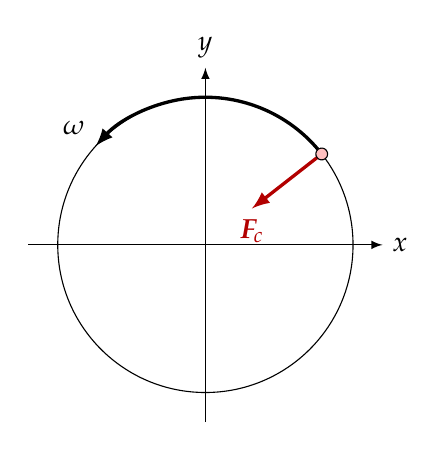
\begin{tikzpicture}[scale=.75]
      \draw[->](-3,0)--(3,0) node[right]{$x$};
      \draw[->](0,-3)--(0,3) node[above]{$y$};
      \draw (0,0) circle(2.5);
      \begin{scope}[rotate=38]
        \begin{scope}[very thick,->]
          \draw[red!70!black] (2.45,0)--(1,0) node[below]{$\bm{F}_c$};
          \draw(2.5,0) arc(0:100:2.5) node[above left]{$\omega$};
        \end{scope}
        \draw[fill=pink] (2.5,0) circle(.1);
      \end{scope}
    \end{tikzpicture}

    \column{.65\textwidth}
    \begin{itemize}
    \item Centripetal force $\bm{F}_c$ is always perpendicular to the
      motion of the object
    \item $\bm{F}_c$ not do any mechanical work
    \item Therefore,  angular velocity $\bm\omega$ remains constant
    \item\textbf{The ``rotational state'' of the object does not change}
    \item Rotation of an object is not determined by merely what forces are
      acting it
    \end{itemize}
  \end{columns}
\end{frame}



\begin{frame}{Turning A Wrench}
  \begin{columns}
    \column{.35\textwidth}
    \pic{1}{wrench}
    
    \column{.65\textwidth}
    Similarly, when tightening/loosening a bolt by turning a wrench.
    \begin{itemize}
    \item When the nut turns, its ``rotational state'' changes
    \item The applied force has to be directed at a distance away from the
      bolt
    \item How easy to turn the nut depends on \emph{both} the distance and the
      force
    \end{itemize}
  \end{columns}
\end{frame}



\begin{frame}{Torque}
  Recall the second law of motion for objects with constant mass:
    
  \eq{-.2in}{
    \bm{F}_\text{net}=m\bm{a}
  }

  \vspace{-.1in}Is it also true for \emph{rotational} motion? If a net force
  $\bm{F}_\text{net}$ causes the center of mass of an object to begin to
  accelerate, what causes a mass to rotate?
\end{frame}


\section{Torque}

\begin{frame}{Torque}
  I have a rod on a table, and with my fingers, I push the two ends of the rod
  with equal force $\textcolor{red!80!black}{F}$. \emph{What happens?}
  \begin{center}
    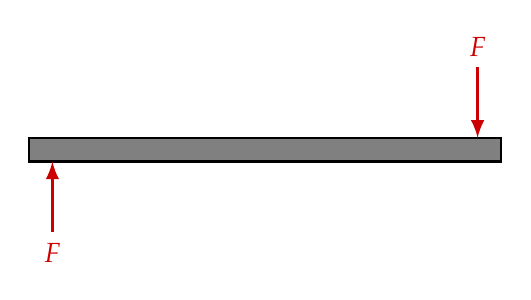
\begin{tikzpicture}[scale=1.5]
      \fill[gray,draw=black,thick] (-2,-.1) rectangle (2,.1);
      \begin{scope}[very thick, red!80!black,<-]
        \draw(-1.8,-.1)--(-1.8,-.7) node[below]{$F$};
        \draw( 1.8, .1)--( 1.8, .7) node[above]{$F$};
      \end{scope}
    \end{tikzpicture}
  \end{center}
  $\bm{F}_\text{net}=\bm{0}$, therefore $\bm{a}=\bm{0}$ at the center of mass.
  But it is also obvious that the rod would \emph{rotate} instead.
\end{frame}



\begin{frame}{What is Torque?}
  \textbf{Torque} (or \textbf{moment}) is the tendency for a force to change
  the rotational motion of a body. The unit for torque is a
  \textbf{newton meter} (\si{\newton\metre}).
  \begin{itemize}
  \item A force $\bm{F}_a$ acting at a point some distance $\bm{r}$ (called the
    \textbf{moment arm}) from a \textbf{fulcrum} (or \textbf{pivot}) at an angle
    $\phi$ between $\bm{F}_a$ and $\bm{r}$
  \item e.g.\ the force to twist a screw
  \item In the example below, a force $\bm{F}$ is applied $\bm{r}$ away from
    the pivot at an angle $\phi$. This generates a torque around the pivot.
  \end{itemize}
  \begin{center}
    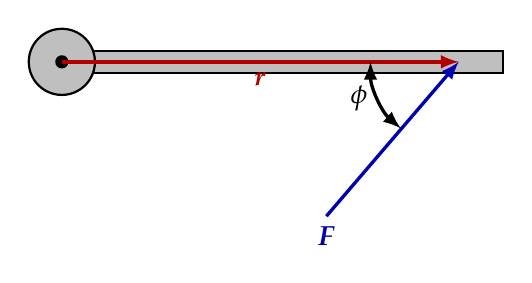
\begin{tikzpicture}[scale=2.8]
      \begin{scope}[thick]
        \draw[fill=gray!50](0,-.05) rectangle (2,.05);
        \draw[fill=gray!50](0,0) circle (.15);
      \end{scope}
      \fill (0,0) circle (.03);
      \begin{scope}[very thick]
        \draw[red!70!black,->](0,0)--(1.8,0) node[midway,below]{$\bm{r}$};
        \draw[blue!70!black,->](1.2,-.7)--(1.8,0) node[pos=0,below]{$\bm{F}$};
        \draw[<->] (1.4,0) arc(180:229:.4)node[midway,left]{$\phi$};
      \end{scope}
    \end{tikzpicture}
  \end{center}
\end{frame}



\begin{frame}{Torque}
  We can express torque $\bm\tau$ in terms of the force $\bm{F}$, the
  \textbf{moment arm} $\bm{r}$ using the cross-product:

  \eq{-.23in}{
    \boxed{\bm{\tau}=\bm{r}\times\bm{F}_a}
  }

  \vspace{-.1in}The magnitude of the torque can be calculated in scalar form
  using the angle $\phi$ between $\bm{F}$ and $\bm{r}$:

  \eq{-.23in}{
    \boxed{\tau=Fr\sin\phi}
  }
  \begin{center}
    \begin{tabular}{l|c|c}
      \rowcolor{pink}
      \textbf{Quantity} & \textbf{Symbol} & \textbf{SI Unit} \\ \hline
      Torque        & $\bm\tau$ & \si{\newton\metre} \\
      Applied force & $\bm{F}_a$  & \si\newton \\
      Moment arm (from fulcrum to force) & $\bm{r}$ & \si\metre \\
      Angle between force and moment arm & $\phi$ & (no units)
    \end{tabular}
  \end{center}
\end{frame}



\begin{frame}{Example Problem}
  \textbf{Example:} Find the net torque on point C.
  \begin{center}
    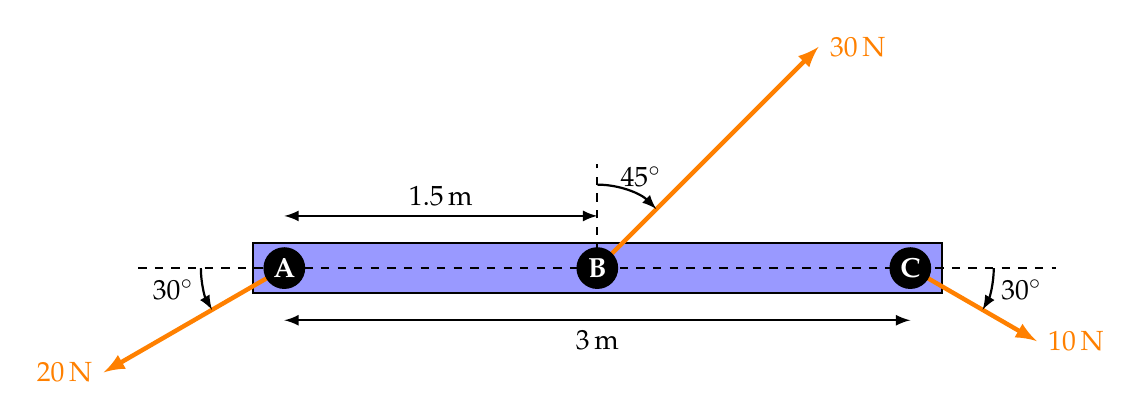
\begin{tikzpicture}[scale=2.65]
      \fill[blue!40,draw=black,thick] (-1.65,-.12) rectangle (1.65,.12);
      \draw[thick,<->](-1.5,-.25)--(1.5,-.25) node[midway,below]{\SI{3.}\metre};
      \draw[thick,<->](-1.5,.25)--(0,.25) node[midway,above]{\SI{1.5}\metre};
      \draw[dashed,thick](-2.2,0)--(2.2,0);
      \draw[dashed,thick](0,0)--(0,.5);
      \begin{scope}[orange,ultra thick,->]
        \draw[rotate=-45](0,0)--(0,1.5)node[right]{\SI{30}\newton};
        \draw[rotate around={30:(-1.5,0)}](-1.5,0)--(-2.5,0)
        node[left]{\SI{20}\newton};
        \draw[rotate around={-30:(1.5,0)}](1.5,0)--(2.2,0)
        node[right]{\SI{10}\newton};
      \end{scope}
      \begin{scope}[thick,->]
        \draw(0,.4)   arc(90:45:.4)  node[pos=.7,above]{\ang{45}};
        \draw(-1.9,0) arc(180:210:.4)node[midway,left] {\ang{30}};
        \draw(1.9,0)  arc(0:-30:.4)  node[midway,right]{\ang{30}};
      \end{scope}
      \fill (-1.5,0) circle(.1);
      \fill (   0,0) circle(.1);
      \fill ( 1.5,0) circle(.1);
      \node[white](A) at (-1.5,0){\textbf{A}};
      \node[white](B) at (0,0)   {\textbf{B}};
      \node[white](C) at (1.5,0) {\textbf{C}};
    \end{tikzpicture}
  \end{center}
%  \uncover<2->{
%    \textbf{Example 8b:} Now find the net torque on A.
%  }
\end{frame}





%\begin{frame}{Torque}
%  Going back to the example question:
%  \begin{center}
%    \begin{tikzpicture}
%      \fill[black!75,draw=black!75] (-5,-.05) rectangle (5,.05);
%      \fill (0,0) circle (.1);
%      \draw[ultra thick](0,0)--(.5,-1.5)--(-.5,-1.5)--(0,0);
%      \uncover<2->{
%        \draw[ultra thick,red!75,->](0,0)--(-4.8,0) node[pos=.5,below]{$d_1$};
%        \draw[ultra thick,red!75,->](-4.8,0)--(-4.8,-1)node[below]{$F_1$};
%      }
%      \uncover<3->{
%        \draw[ultra thick,blue!60,->](0,0)--(4,0) node[pos=.5,below]{$d_2$};
%        \draw[ultra thick,blue!60,->](4,0)--(4,-1.2) node[below]{$F_2$};
%      }
%    \end{tikzpicture}
%  \end{center}
%  \begin{itemize}
%  \item<2->$F_1$ will rotate the board counter clockwise
%  \item<3->$F_2$ will rotate the board clockwise
%  \item<4->The beam will remain static (in equilibrium) if
%
%    \eq{-.2in}{ F_1d_1=F_2d_2 }
%  \end{itemize}
%\end{frame}



\section{Angular Momentum}

\begin{frame}{Angular Momentum}
  Consider a mass $m$ connected to a massless beam rotates with speed $v$ at
  a distance $r$ from the center (shown on the right). It has an
  \textbf{angular momentum} ($\bm{L}$), defined as:
  \begin{columns}
    \column{.77\textwidth}
    
    \eq{-.32in}{
      \boxed{\bm{L}=\bm{r}\times\bm{p}=m(\bm{r}\times\bm{v})}%=mr^2\bm\omega}
    }

    \vspace{-.1in}Expanding the term with $\bm{v}=\bm\omega\times\bm{r}$, the
    expression for angular momentum can now be expressed in quantities related
    to rotations:

    \eq{-.32in}{
      \boxed{\bm{L}=m(\bm{r}\times\bm{v})
        =m(\bm{r}\times(\bm\omega\times\bm{r}))
        =mr^2\bm\omega}
    }
    
    \vspace{-.2in}Or in scalar form:
    
    \eq{-.25in}{
      \boxed{L=rmv=mr^2\omega}
    }

    \vspace{-.2in}The unit for angular momentum is a
    \textbf{kilogram meter squared per second}
    (\si{\newton\metre\squared\per\second}).
    
    \column{.23\textwidth}
    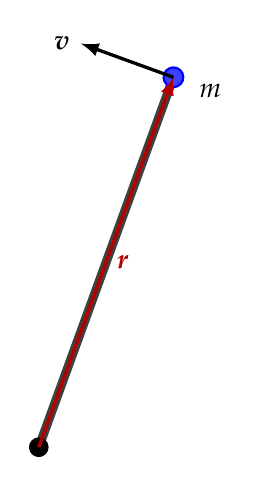
\begin{tikzpicture}[scale=2.5]
      \begin{scope}[rotate=70]
        \fill[black!75,draw=black!75] (0,-.02) rectangle (2,.02);
        \fill[blue!75,draw=blue,thick] (2,0) circle(.05);
        \node(M) at (2,-.2) {$m$};
        \fill (0,0) circle (.05);
        \begin{scope}[very thick,->]
          \draw[red!70!black](0,0)--(2,0)node[midway,right]{$\bm{r}$};
          \draw (2,0)--(2,.5)node[left]{$\bm{v}$};
        \end{scope}
      \end{scope}
    \end{tikzpicture}
  \end{columns}
\end{frame}



\begin{frame}{Moment of Inertia}
  Look again at the definition of angular momentum:
    
  \eq{-.2in}{
    \bm{L}%=\bm{r}\times\bm{p}=\bm{r}\times(m\bm{v})
    %=m\bm{r}\times(\bm{\omega}\times\bm{r})
    =\underbrace{mr^2}_{I}\bm\omega
  }
    
  The quantity $I=mr^2$ is called the \textbf{moment of inertia} with a unit of
  \textbf{kilogram meter squared} (\si{\kilo\gram\metre\squared}), and 

  \eq{-.2in}{
    \boxed{\bm{L}=I\bm\omega}
  }

  Momentum of inertia can be considered to be an object's ``rotational mass''

\end{frame}



\begin{frame}{Moment of Inertia}
  For a \emph{single particle} of $m$ rotating at a distance $r$ from the pivot:
  
  \eq{-.2in}{
    \boxed{I=mr^2}
  }

  For a \emph{collection of particles}, each of mass $m_i$ at distance $r_i$
  from the pivot:

  \eq{-.2in}{
    \boxed{I=\sum m_ir_i^2}
  }

  For a \emph{continuous distribution of mass} about a pivot, integral calculus
  is need to calculate the momentum of inertia\footnote{don't worry, no one
    will ask you to do this in this course!}

  \eq{-.25in}{
    \boxed{I=\int r^2dm}
  }
\end{frame}



\begin{frame}{Moment of Inertia}
  \centering
  \pic{.7}{mic}
\end{frame}



\begin{frame}{Angular Momentum and Moment of Inertia}
  Linear and angular momentum have very similar expressions
    
  \eq{-.2in}{
    \boxed{\bm{p}=m\bm{v}}\quad\quad\quad\boxed{\bm{L}=I\bm\omega}
  }
  
  Just as $\bm{p}$ describes the overall \emph{translational} state of a
  physical system, $\bm{L}$ describes its overall \emph{rotational} state
\end{frame}



\section{Laws of Motion}

\begin{frame}{Equilibrium: First Law of Motion}
  An object is in \textbf{translational equilibrium} is when the net force
  acting on it is zero:
  
  \eq{-.2in}{
    \bm{F}_\text{net}=\bm{0}
  }

  This does \emph{not} mean that the object has no translational motion; it
  just means that the object's overall \emph{transtational state} is not
  changing, i.e.\ the translational momentum $\bm{p}$ is constant. For
  constant mass, this means $\bm{a}=\bm{0}$.
\end{frame}




\begin{frame}{Equilibrium: First Law of Motion}
  Likewise, an object is in \textbf{rotational equilibrium} when the net torque
  acting on it is zero:

  \eq{-.3in}{
    \bm{\tau}_\text{net}=\bm{0}
  }
  
  This does \emph{not} mean that the object has no rotational motion; it just
  means that the object's overall \emph{rotational state} is not changing,
  i.e.\ $\bm{\alpha}=\bm{0}$, or that the angular momentum $\bm{L}$ is constant.
\end{frame}



\begin{frame}{Second Law of Motion for Rotational Motion}
  The net torque is the time rate of change of angular momentum:

  \eq{-.2in}{
    \bm{\tau}_\text{net}=\bm{r}\times\bm{F}_\text{net}
    =\bm{r}\times\frac{d\bm{p}}{dt}
    =\frac{d(\bm{r}\times\bm{p})}{dt}\;\;\longrightarrow\;\;
    \boxed{\bm{\tau}_\text{net}=\frac{d\bm{L}}{dt}}
  }
  \begin{itemize}
  \item If the net torque on a system is zero, then the rate of change
    of angular momentum is zero, and we say that the angular momentum is
    conserved. 
  \item e.g.\ When an ice skater starts to spin and draws his arms inward.
    Since angular momentum is conserved, a decrease in $r$ means an
    increase in $\omega$.
  \end{itemize}
\end{frame}



\begin{frame}{Second Law of Motion}
  For translational motion, the general form of the first and second laws of
  motion states that the net force is rate of change of the object's momentum:

  \eq{-.2in}{
    \bm{F}_\text{net}=\frac{d\bm{p}}{dt}
  }

  For objects with constant mass, the second law reduces to the more familiar
  form:

  \eq{-.2in}{
    \bm{F}=m\bm{a}
  }
\end{frame}



\begin{frame}{Second Law of Motion for Rotational Motion}
  Likewise, the second law of motion for rotational motion has a similar
  form, but with torque $\bm\tau$ replacing force $\bm{F}$, and angular
  momentum $\bm{L}$ replacing linear momentum $\bm{p}$:

  \eq{-.2in}{
    \boxed{
      \bm{\tau}_\text{net}=\frac{d\bm{L}}{dt}
    }
  }

  For objects with constant momentum of inertia $I$, the second law of motion
  reduces to:

  \eq{-.2in}{
    \bm\tau_\text{net}=I\bm\alpha
  }
\end{frame}



\begin{frame}{But there is no rotational motion, is there?}
  Even when there is no apparent rotational motion, it does not necessarily
  mean that angular momentum is zero! In this case, mass $m$ travels along a
  straight path at constant velocity (uniform motion), but the angular momentum
  around point $P$ is not zero:
  \begin{center}
    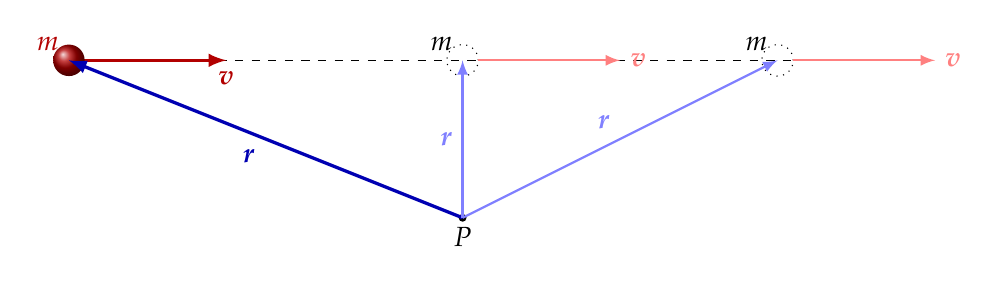
\begin{tikzpicture}
      \draw[dashed](-5,0)--(5,0);
      \draw[very thick,red!70!black,->](-5,0)--(-3,0) node[below]{$\bm{v}$};
      \tikzstyle{balloon}=[ball color=red!70!black];
      \shade[balloon] (-5,0) circle(.2) node[above left,red!70!black]{$m$};
      \fill (0,-2) circle(.05) node[below]{$P$};
      \draw[very thick,blue!70!black,->](0,-2)--(-5,0)
      node[midway,below left]{$\bm{r}$};
      \uncover<2->{
        \draw[dotted](0,0) circle(.2) node[above left]{$m$};
        \draw[thick,red!50,->](.2,0)--(2,0)node[right]{$\bm{v}$};
        \draw[thick,blue!50,->](0,-2)--(0,0) node[midway,left]{$\bm{r}$};
      }
      \uncover<3->{
        \draw[dotted](4,0) circle(.2) node[above left]{$m$};
        \draw[thick,red!50,->](4.2,0)--(6,0)node[right]{$\bm{v}$};
        \draw[thick,blue!50,->](0,-2)--(4,0)node[midway,above left]{$\bm{r}$};
      }
    \end{tikzpicture}
  \end{center}
  \uncover<4>{
    Since there is no force and no torque acting on the object, both the linear
    momentum ($\bm{p}=m\bm{v}$) and angular momentum
    ($\bm{L}=\bm{r}\times\bm{v}$) are constant.
  }
\end{frame}



\begin{frame}{Example Problem}
  \textbf{Example:} A skater extends her arms (both arms!), holding a
  \SI{2.}{\kilo\gram} mass in each hand. She is rotating about a vertical axis
  at a given rate. She brings her arms inward toward her body in such a way that
  the distance of each mass from the axis changes from \SI{1.}\metre to
  \SI{.50}\metre. Her rate of rotation (neglecting her own mass) will?
\end{frame}




\begin{frame}{Example Problem}
  \textbf{Example:} A \SI{1.}{\kilo\gram} mass swings in a vertical circle
  after having been released from a horizontal position with zero initial
  velocity. The mass is attached to a massless rigid rod of length
  \SI{1.5}\metre. What is the angular momentum of the mass, when it is in its
  lowest position?
\end{frame}



\begin{frame}{Solving Rotational Problems}
  When solving for rotational problems like the ones described in the previous
  sections:
  \begin{itemize}
  \item Draw a free-body diagram to account for all forces
  \item The direction of friction force is not always obvious
  \item The magnitude of any static friction force cannot be assumed to be at
    maximum.
  \item If the object is to change its rotational state, there must be a net
    torque causing it.
  \end{itemize}
\end{frame}



\begin{frame}{Solving Rotational Problems}
  Once the free-body diagram is complete
  \begin{itemize}
  \item Breaks down the \emph{forces} into $\iii$, $\jjj$ and $\kkk$ components
  \item We have now three equations for translation, but it is likely that only
    \emph{one} direction will have forces:

    \eq{-.3in}{
      \sum F_x=ma_x\quad\quad \sum F_y=ma_y\quad\quad \sum F_z=ma_z
    }
  \item And three equations for rotation, and torque is only applied in one
    direction (likely $\kkk$):
    
    \eq{-.3in}{
      \sum\tau_x=I_x\alpha_x\quad\quad \sum\tau_y=I_y\alpha_y\quad\quad 
      \sum\tau_z=I_z\alpha_z
    }
  \end{itemize}
\end{frame}



\begin{frame}{Solving Rotational Problems}
  For rotational motion dynamics equation:
  \begin{enumerate}
  \item Relate the force(s) that causes rotational motion to the net torque

    \eq{-.2in}{
      \tau=Fr
    }
  \item Substitute the expression for momentum of inertia (which has both mass
    and radius terms in it) into the equation for rotational motion
  \item Relate angular acceleration to linear acceleration, if applicable:

    \eq{-.25in}{
      \alpha=\frac{a}R
    }
  \end{enumerate}
  Now there are two equations with force and acceleration terms. See handout
\end{frame}


  
\section{Work \& Energy in Rotational Motion}

\begin{frame}{Mechanical Work}
  For translational motion, mechanical work is defined as

  \eq{-.2in}{
    W=\int_{x_1}^{x_2}\bm{F}\cdot d\bm{x}
  }

  For rotational motion, mechanical work is defined similarly as:

  \eq{-.2in}{
    \boxed{
      W=\int_{\theta_1}^{\theta_2}\bm\tau\cdot d\bm\theta
    }
  }

  The work-energy theorem still applies to rotational motion, i.e.;

  \eq{-.25in}{
    W=\Delta K
  }
\end{frame}


\begin{frame}{Rotational Kinetic Energy}
  To find the kinetic energy of a rotating system of particles (discrete number
  of particles, or continuous mass distribution), we sum the
  kinetic energy of the individual particles:
    
  \eq{-.1in}{
    K=\sum_i\frac12m_iv_i^2=\frac12\left(\sum_i m_ir_i^2\right)\omega^2
  }
  
  It's no surprise that in both case, rotational kinetic energy is given by:
  
  \eq{-.2in}{
    \boxed{K=\frac12I\omega^2}
  }
\end{frame}



\begin{frame}{Kinetic Energy of a Rotating System}
  The total kinetic energy of a rotating system is the sum of its translational
  and rotational kinetic energies at its center of mass:

  \eq{-.2in}{
    \boxed{K=\frac12mv_\text{CM}^2+\frac12I_\text{CM}\omega^2}
  }
  
  In this case, $I_\text{CM}$ is calculated at the center of
  mass. For simple problems, we only need to compute rotational kinetic energy
  at the pivot:

  \eq{-.2in}{
    \boxed{K=\frac12I_\text{P}\omega^2}
  }
  
  In this case, the $I_\text{P}$ is calculated at the pivot.
  \textbf{IMPORTANT:} $I_\text{CM}\neq I_\text{P}$
\end{frame}



%TL1\begin{frame}{Parallel Axis Theorem}
%TL1  \begin{columns}
%TL1    \column{.35\textwidth}
%TL1    \pic{1}{Steiner.png}
%TL1    
%TL1    \column{.65\textwidth}
%TL1    The \textbf{parallel axis theorem} relates the moment of inertia of an
%TL1    object along two different but parallel axis by:
%TL1
%TL1    \eq{-.2in}{
%TL1      \boxed{I=I_{\textrm{CM}}+md^2}
%TL1    }
%TL1  \end{columns}
%TL1\end{frame}
\end{document}
